%----------------------------------------------------------------------------
\chapter{Implementation}
%----------------------------------------------------------------------------
\section{Different versions of NI LabVIEW}
At the time of writing this thesis, National Instruments offers two versions of LabVIEW: LabVIEW 2018\footnote{\url{http://www.ni.com/en-us/shop/labview/labview-details.html}}, and LabVIEW NXG\footnote{\url{http://www.ni.com/en-us/shop/labview/labview-nxg.html}}. LabVIEW 2018 is a sequel to the LabVIEW versions released in the past few years, it operates reliably and fast, has support for all the NI hardware, and has a wide range of features. LabVIEW NXG is a brand new product, it has been created from scratch, and has been developed according to current standards - optimized for the newest hardware and software, and a really comfortable UI. Most features are still beta however, or under development\footnote{\url{http://www.ni.com/pdf/products/us/labview-roadmap.pdf}}, a large number of hardware are not yet supported, and the operation is not as reliable as the current generation software.\cite{nxg_article}

LabVIEW 2018 and LabVIEW NXG are not really compatible with each other, though the interface and the programming is similar, they have completely different execution engines and file formats. There is a tool bundled with NXG for current generation project conversion, but it is not perfect, and almost always the converted VIs need manual fixing afterwards.

Given two distinct LabVIEW products, it has to be decided which to develop the tool for. Both of them have advantages: current generation LabVIEW has a larger user base than NXG, but developing for NXG will make the tool compatible with actual software for a longer time (since NXG will eventually replace current generation LabVIEW).
\subsection{Comparing the API}
For making a decision on the LabVIEW version, the main point was the method of integrating the tool into LabVIEW. 

Reading the VI data from file is quite difficult. The file format definition of current generation VIs is not published, so the only software that can read the file is LabVIEW. NXG stores the VI data in XML files, which is a lot friendlier. It is possible to create an interpreter, and build the object model, since the nodes are XML elements, and the connections are made using unique identifiers.

Building a plugin is an option too. LabVIEW 2018 has a toolbox called VI Scripting\footnote{\url{http://sine.ni.com/nips/cds/view/p/lang/en/nid/209110}} for G language. It has several commands to access or modify VI object models and project structure. Project Provider Framework\footnote{\url{http://www.ni.com/white-paper/13921/en/}} allows an add-on to be integrated into the interface of LabVIEW, like creating a menu command or a toolbar button.

A plugin for LabVIEW NXG needs a different approach. Most of NXG uses .NET framework, and an add-on integrates in a form of a .NET class library (DLL). The object model of a Virtual Instrument is directly accessible as a .NET object, and plugin entry points can easily be defined with class attributes. UI elements can be easily created as well. This way, the plugin is written in C\# language.

I have chosen to create an NXG plugin, since writing such a complex tool in G language would require such an expertise in LabVIEW, that I do not have. Additionally, I already had the routine in NXG API and C\#.
\section{LabVIEW NXG API and object model}
There is hardly any documentation on the NXG programming interface at the moment, but an example plugin project on GitHub\footnote{\url{https://github.com/ni/nidevlabs}}. Fortunately, this project had almost all the API I needed for this project.
\lstset{escapechar=@}
\begin{lstlisting}[frame=single,escapechar=@,float=!ht,caption={NXG plugin entry point},captionpos=b,label={lst:menuapi},language=C++]
[ExportPushCommandContent]
public class LauncherCommands : PushCommandContent
{
    public static readonly ICommandEx SymbolicMenuRoot = new RelayCommandEx(RelayCommandEx.HandleNoOp)
    {
        UniqueId = "SymbolicTool.MenuRoot",
        LabelTitle = "SymbolicTool",
        MenuParent = MenuPathCommands.RootMenu
    };
    public readonly ICommandEx RunCommand = new ShellRelayCommand(OnRun)
    {
        UniqueId = "SymbolicTool.RunCommand",
        LabelTitle = "Run Symbolic Execution",
        MenuParent = SymbolicMenuRoot
    };
    public override void CreateApplicationContent(ICommandPresentationContext context)
    {
        base.CreateApplicationContent(context);
        context.Add(SymbolicMenuRoot);
        context.Add(RunCommand);
    }
    public static void OnRun(ICommandParameter parameter, ICompositionHost host, DocumentEditSite site)
    {
        // Run the program here
    }
}
\end{lstlisting}

\begin{figure}

\centering
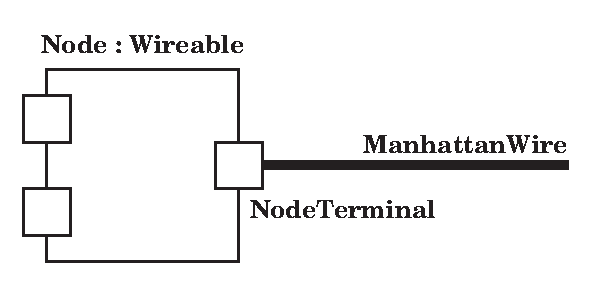
\includegraphics[width=80mm,keepaspectratio]{figures/lvobject.pdf}
\caption{LabVIEW Node object model} 
\label{fig:lvobject}
\end{figure}
I implemented a launcher code based on the ExamplePlugins project, that integrates a menu command into the menu bar of NXG (Listing \ref{lst:menuapi}). The three parameters of the callback function provide access to the object model of LabVIEW. DocumentEditSite refers to the currently opened document, and since the execution will run on the opened VI, getting the model will be really easy: \lstinline[columns=fixed]{rootElement = site.ActiveDocumentEditor?.EditorInfo?.RootElement;}. The model will be passed to the parser component, then the returned Sequence object (which holds the procedural program) is given to the symbolic execution module (Listing \ref{lst:launchercode}). When finished, values of symbolic variables will be placed in each leaf, and can be retrieved using a \lstinline[columns=fixed]{leaf.getSymbols()} call.
\lstset{escapechar=@}
\begin{lstlisting}[frame=single,escapechar=@,float=!ht,caption={Launcher code},captionpos=b,label={lst:launchercode},language=C++]
public static void OnRun(ICommandParameter parameter, ICompositionHost host, DocumentEditSite site)
{
    var rootElement = site.ActiveDocumentEditor?.EditorInfo?.RootElement;
    if (rootElement == null) return;
    var sequence = VIConverter.VIConverter.CreateModel(rootElement);
    Symbolic.SymbolicExec se = new Symbolic.SymbolicExec(sequence.getStatements());
    List<Symbolic.ExecutionState> leafs = se.Execute();
    // Print symbolic variable values
}
\end{lstlisting}
\section{The parser}
The algorithm used in the main parser loop is a sort of breadth-first search. The nodes waiting to be processed get placed in a queue object (which initializes with those nodes, that have no input wires, and can be executed right away). The main loop takes a node from the front of the queue, and makes sure all its input nodes are already processed - this is important, because at the end of processing a node, all the output nodes are added to the queue, and they not necessarily have all their inputs ready. 

A \textit{Statement}\footnote{Note: the classes of my implementation are indicated with \textit{italic}, the classes of LabVIEW API are indicated with \underline{underlined} font} is created for the node, then the arithmetical, logical or other operations are added respectively: an \textit{Expression} (which can be as simple as an addition, or a more complex expression, a nested structure of \textit{Operator}s) placed in an \textit{Assignment}, which assigns the \textit{Expression} value to a \textit{Variable}. When the node is a \underline{DataAccessor} (LabVIEW control), a \textit{SymbolicVariable} will be introduced.


\begin{algorithm}
\ForEach{nodes of rootElement without input wires}{
add node to nextNodes\;
}
\If{rootElement is NestedDiagram}{
\ForEach{input tunnels}{
add output nodes to nextNodes\;
}
}
\While{nextNodes is not empty}{
thisNode:=nextNodes.Dequeue\;
\eIf{thisNode has all inputs ready}{
statement:=new Statement\;
inputVariables:=variableDictionary[input wires of thisNode]\;
\ForEach{output wires of thisNode}{
variableDictionary[output wire]:=new Variable\;
}
\Switch{type of thisNode}{
\uCase{SourceModel.Add}{statement.addOperation(createAssignment(outputVariables[0], createAddition(inputVariables[0], inputVariables[1])))\;}
\uCase{SourceModel.Multiply}{statement.addOperation(createAssignment(outputVariables[0], createMultiplication(inputVariables[0], inputVariables[1])))\;}
\vspace{2mm}
...\\
\uCase{SourceModel.Literal}{statement.addOperation(createAssignment(outputVariables[0], createConstant(thisNode.Data)))\;}
\uCase{SourceModel.DataAccessor}{statement.addOperation(createAssignment(outputVariables[0], createSymbolicVariable(thisNode.DataItemName)))\;}
\Case{SourceModel.BorderNode}{
\If{thisNode.Owner is CaseStructure and all its inputs are ready}{
create variables for all input and output tunnels\;
statement:=new IfStatement\;
statement.trueBranch:=Parser(true diagram)\;
statement.falseBranch:=Parser(false diagram)\;

}
}
}
sequence.add(statement)\;
\ForEach{follow output wires of thisNode}{
nextNodes.Enqueue(found node)\;
}
}{
nextNodes.Enqueue(thisNode)\;
}

}
 \caption{A simplified algorithm of Parser(rootElement)}
 \label{alg:parser}
\end{algorithm}

The parser binds a \textit{Variable} to all of the wires. New \textit{Variable}s are introduced, when the parser processes the output wires of a node (since a wire can be connected to only one node output), and all \underline{ManhattanWire} - \textit{Variable} pairs will be stored in a lookup table (C\# Dictionary) global to a single run of the algorithm. This way, if multiple nodes use that output as an input, it will be the same \textit{Variable}.

When the search reaches a case structure, the parser will be recursively called for both subdiagrams. Wires enter the case diagram through \underline{BorderNode}s (or tunnels), so that for each of them a new \textit{Variable} will be introduced. In a subdiagram, the search will start from the \underline{BorderNode}s (and the nodes without input wires). After the search execution for both diagrams, the execution returns to the root parser.

To summarize, the simplified pseudo-code is listed in Algorithm \ref{alg:parser}, that is easier to understand than the original source. 
The explanation of data structures used during the operation of the parser:

\begin{itemize}
\item \textbf{rootElement} : \underline{Element} -- the parameter of the algorithm, the diagram, whose immediate child nodes must be searched
\item \textbf{nextNodes} : Queue<\underline{Wireable}> -- found \underline{Nodes}, waiting to be processed
\item \textbf{variableDictionary} : Dictionary<\underline{ManhattanWire}, \textit{Variable}> -- association between LabVIEW wires and variables in the procedural program
\item \textbf{sequence} : \textit{Sequence} -- the procedural program, chain of \textit{Statement}s, the result of this algorithm
\end{itemize}



Of course, this pseudo-code is more of a demonstration, than the actual program. A number of workaround solutions had to be used to handle special cases in the block diagram. For instance, when a case structure had two output tunnels, that connect to one source in the subdiagram, two variables were created for the same wire, which is invalid. The second variable had to be assigned the value of the first variable.

Since references from one LabVIEW object to another were mostly using a heterogenous collection, type checks and type casts take up a large percentage of the source code.

\section{Symbolic Execution Loop}

As mentioned earlier, symbolic execution is an extension to regular execution. The loop will iterate through the program, and execute the statements as it would normally, if there are no symbolic variables present.

The current execution environment is stored in an \textit{ExecutionState} object. This object stores the calculated values of \textit{Variable}s and the path condition throughout the execution. If the value of a variable is calculated from a symbolic variable, an \textit{Expression} containing the \textit{SymbolicVar} gets stored. It is important, that these values never store a reference to another \textit{Variable} object, when evaluating such an expression, since these might change after assignment, and the values would become invalid. During evaluation, the stored value of the \textit{Variable} is substituted into the expression, and if the two operands of an \textit{Operator} are constant values, the corresponding operator can evaluate with their values (see Listings \ref{lst:operator_eval} and \ref{lst:variable_eval}). 

\begin{lstlisting}[frame=single,escapechar=@,float=!ht,caption={Evaluation part of the Operator class},captionpos=b,label={lst:operator_eval},language=C++]
class Operator : Expression
{
    Expression A { get; set; }
    Expression B { get; set; }
    string Op { get; set; }
    
    // ...
    
    public override Expression Evaluate(ExecutionState es)
    {
        Expression a = A.Evaluate(es);
        Expression b = null; // for expressions with only one operand
        if (B!=null)b = B.Evaluate(es);
        if (a is Constant && b is Constant)
        {
            switch (Op)
            {
                case "+":
                    return new Constant((a as Constant).Value + (b as Constant).Value);
                // ...
            }
        }
        // ...
        return new Operator(a, b, Op);
    }
}
\end{lstlisting}

\begin{lstlisting}[frame=single,escapechar=@,float=!ht,caption={Evaluation part of the Variable class},captionpos=b,label={lst:variable_eval},language=C++]
class Variable : Expression
{
    string Name { get; set; }

    // ...
    
    public override Expression Evaluate(ExecutionState es)
    {
        return es.GetVariableValue(this);
    }
}
\end{lstlisting}

\begin{lstlisting}[frame=single,escapechar=@,float=!ht,caption={The part of ExecutionState related to execution},captionpos=b,label={lst:executionstate},language=C++]
class ExecutionState
{
    public Dictionary<Variable, Expression> variableValues = new Dictionary<Variable, Expression>();
    public Expression Pc;

    // ...

    public Expression GetVariableValue(Variable v)
    {
        return variableValues[v];
    }
    public void SetVariableValue(Variable v, Expression e)
    {
        variableValues[v] = e;
    }
    public ExecutionState Clone()
    {
        return new ExecutionState(new Dictionary<SymbolicVar, Expr>(symbolicVariables), new Dictionary<Variable, Expression>(variableValues), Pc);
    }

    public ExecutionState(Dictionary<SymbolicVar, Expr> symbolicVariables, Dictionary<Variable, Expression> variableValues, Expression pc)
    {
        this.symbolicVariables = symbolicVariables;
        this.variableValues = variableValues;
        Pc = pc;
    }
    // ...
}

\end{lstlisting}

The interesting part is handling \textit{IfStatement}s. The true and false branches of the structure are stored in the object as \textit{Sequence}s, therefore a new execution can be started for each of them. 

Before doing that, it must be verified, if the path condition extended with the condition of the if statement (or its negate for the false branch) is satisfiable or not. (For doing that the constraint solver will already be used. It will be described in the later sections, how \textit{Expression}s are getting handed to the solver.) If it is satisfiable, the execution state gets cloned for each branch, and updated with the extended path conditions. 

At this point, the operation of the tool resembles a depth-first search algorithm: the execution of the two execution branches begin right away, one after another, and each gets the program sequence from their part of the if statement, plus the rest of the program after the if statement. This way, the remaining part of the program will run twice, in the context of both branches.

When the run comes to the end, the routine returns the \textit{ExecutionState} of the finished program. This \textit{ExecutionState} (possibly) gets returned to the evaluation to the if statement, where these states are added to a list, and after executing both branches, the routine returns with the list. 

It can be seen, that calling the symbolic execution routine on the sequence of the entire program will return a list of \textit{ExecutionState}s of all possible execution paths (these are the leafs of the execution tree). These all have their own path condition, which now can be evaluated by the solver, to get the input values for each of them.

\section{Running the solver}
At the end of execution, \textit{ExecutionState} objects will contain a path condition (\textit{Expression}), which consist of symbolic variables, constant values, and operators. These kind of formulas are the constraints, the solver is expecting, it just needs to be translated to its own language. 

The object model of the solver is really similar to the \textit{Expression} model used in the tool. All of the \textit{Expression} classes get a \lstinline[columns=fixed]{Microsoft.Z3.Expr BuildTerm(Context ctx, ExecutionState es);} function, which builds the Z3 expression recursively. The needed symbolic variables are defined during this conversion (and are stored in \textit{ExecutionState}, for not to redefine in the case of multiple usage). The relevant parts are listed in Listing \ref{lst:executionstate_solver}.


\begin{lstlisting}[frame=single,escapechar=@,float=!ht,caption={Calling the solver in ExecutionState},captionpos=b,label={lst:executionstate_solver},language=C++]
class ExecutionState
{
    // ...
    public Dictionary<SymbolicVar, Expr> symbolicVariables = new Dictionary<SymbolicVar, Expr>();
    // ...
    public Expression Pc;

    public Expr GetSymbolicVariable(SymbolicVar s, Context ctx, Sort range=null)
    {
        if (symbolicVariables.ContainsKey(s))
        {
            return symbolicVariables[s];
        }
        else
        {
            if (range == null) range = ctx.MkIntSort();
            Expr e = ctx.MkConst(s.Name, range);
            symbolicVariables.Add(s, e);
            return e;
        }
    }
    // ...
    private Solver GetSolver()
    {
        if (Pc == null) Pc = new BoolConstant(true);
        using (Context ctx = new Context())
        {
            symbolicVariables.Clear();
            Expr pathCondition = Pc.BuildTerm(ctx, this);
            Solver s = ctx.MkSolver();
            s.Assert((BoolExpr)pathCondition);
            return s;
        }
    }
    public bool CheckModel()
    {
        Solver s = GetSolver();
        return s.Check().ToString().Equals("SATISFIABLE");
    }
    public Dictionary<string, string> GetSymbols()
    {
        Dictionary<string, string> symbols = new Dictionary<string, string>();
        Solver s = GetSolver();
        var check = s.Check();
        Microsoft.Z3.Model m = s.Model;
        foreach(FuncDecl d in m.Decls)
        {
            symbols.Add(d.Name.ToString(), m.ConstInterp(d).ToString());
        }
        return symbols;
    }
}

\end{lstlisting}

\section{Displaying the output}
For this is only a prototype, the results, which are the list of execution paths, their path conditions, and the calculated symbolic variables. After getting the execution tree leafs (see Listing \ref{lst:launchercode}), a simple string builder loop collects the data from the output structures, and the final string gets displayed in a \underline{NIMessageBox}.